% !TEX encoding = UTF-8 Unicode
\kap{Installation}
\ukap{System requirements}
\uukap{Windows}
        \begin{itemize}
	\item Windows XP(SP3)/Vista/7  
        \item Pentium/Athlon Prozessor 500Mhz or better
	\item 512MB RAM
	\item about 20MB free disk space
	\item Windows XP(SP3)/Vista/7 compatible soundcard
	\item a host application with VST2.x support
	\end{itemize}
%\uukap{Mac}
%	\begin{itemize}
%        	\item Apple PowerPC/i386 500Mhz oder schneller
%		\item 512MB RAM
%		\item 40MB freier Speicherplatz auf der Festplatte
%		\item Core-Audio kompatible Audioschnittstelle
%		\item MacOs 10.4.0 oder höher
%		\item Eine VST2.x kompatible Hostanwendung
%	\end{itemize}
%\uukap{\label{compatible}Unterstützte Pluginformate}
%Derzeit wird lediglich das VST2.x Pluginformat in der 32-bit Variante unterstützt.
\newpage
\ukap{Installation}
Just extract the whole content of the .zip file into the vst-plugin folder of your host application. 
Open the host application and check that VSTForx was loaded successfully.
You should find two VSTForx plugin variants:
\begin{itemize}
	\item vstforx (the effect)
	\item vstforxInstrument (the instrument)
\end{itemize}

\ukap{Configuration}
\begin{figure}[h]
\begin{center}
	
\includegraphics[scale=0.3]{../graphics/disco_main_view}
\caption{the editor}
\label{blank}
\end{center}
\end{figure}

Load VSTForx into your host application. Open the editor (figure \ref{blank}). \\
To open the setup dialog use the \emph{''Open Setup Dialog''} entry in the context menu of the main view.

\begin{figure}[h]
\begin{center}
	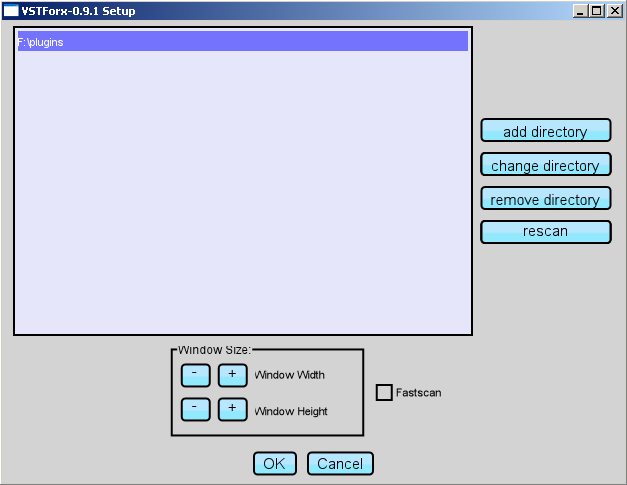
\includegraphics[scale=0.4]{../graphics/disco_setup}
\caption{the setup dialog}
\label{setup}
\end{center}
\end{figure}

\uukap{\label{scanconfig}The Scan}
\paragraph{Adding Pluginfolders}
With the buttons \emph{'add Directory'}, \emph{'change Directory'} and \emph{'remove Directory'}
you are able to configure the search folders of the VSTForx database.

\paragraph{The Scan Process} 
While the scanning process, VSTForx searches the given folders for VST plugins. Depending on the number of plugins the scan process may take a while. An extra window will show you the results of the current scan (figure \ref{scanres}).
\\\\

\textbf{Heads Up: don't forget to repeat this process when your plugin folder content has changed!}
\begin{figure}[h]
\begin{center}
	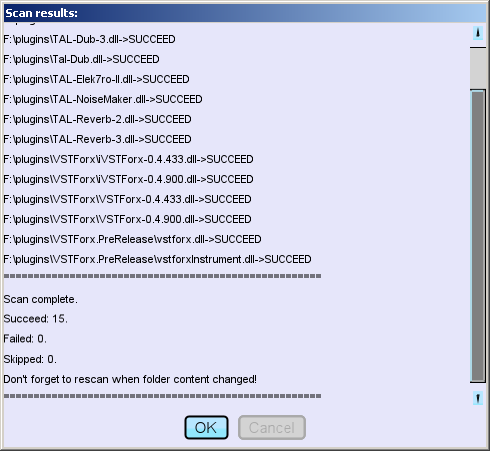
\includegraphics[scale=0.3]{../graphics/scan_result}
\caption{the scan result window}
\label{scanres}
\end{center}
\end{figure}
\paragraph{Fast Scan}
Is the \emph{''fast scan''} option activated, the scan process recognizes a plugin only with the filename.
The scan process is faster now but there is a lack of detailed informations about the scanned plugins (e.g. is it a instrument or not). Besides that there is a risk of recognizing a system .dll as a plugin.

\uukap{Window Options}
With the \emph{''Window Size''} buttons you are able to change the editor size of the VSTForx editor.  

